% =============================================================
% Methodology section -- magnetically actuated continuum beam.
% IEEEtran (journal). Standalone compilable excerpt: the full
% paper supplies title/abstract/introduction/experiments/
% validation/discussion. Section numbering renumbers on merge.
%
% Bibliography entries carry short "% VERIFY" notes where the
% volume/issue/page/DOI fields still need completing.
% =============================================================
\documentclass[journal]{IEEEtran}

\usepackage{amsmath}
\usepackage{amssymb}
\usepackage{amsfonts}
\usepackage{graphicx}
\usepackage{booktabs}
\usepackage{tikz}
\usetikzlibrary{arrows.meta,positioning}

\begin{document}

\section{Methodology}
\label{sec:methodology}

\subsection{Problem Formulation and Assumptions}
\label{sec:problem}

A flexible, permanently magnetized beam is advanced through a fixed
insertion point while a permanent magnet, carried by the end-effector of a
six-axis manipulator, shapes it through magnetic interaction. Given a
desired tip trajectory $p^\star(t)$, the control problem is to select the
manipulator joint velocities and the insertion rate that drive the
measured beam tip along $p^\star(t)$, subject to the manipulator's
velocity, acceleration and joint-range limits, using only the beam shape
observed by an external camera.

The models developed below rest on five assumptions, stated here once and
used throughout.

\begin{enumerate}
\item[(A1)] \emph{Quasi-static beam response.} The beam is assumed to
reach mechanical equilibrium quickly relative to the control period, so
its shape at each control instant is the static energy minimizer for the
instantaneous magnet pose. This is the standard modeling choice for
magnetically steered elastic rods and catheters at the actuation
bandwidths considered here~\cite{kratchman2017guiding,wu2025closedloop}.
\item[(A2)] \emph{Hard magnetization.} The beam carries a fixed
(hard-magnetized) magnetic moment density, specified in the body frame and
unchanged by the applied field; no induced or field-dependent
magnetization is modeled.
\item[(A3)] \emph{Point-dipole source.} The actuating magnet is modeled as
an ideal point dipole, valid at the beam--magnet separations used here.
\item[(A4)] \emph{Planar deformation.} The beam is calibrated to deform
within a single plane, which the vision pipeline of
Sec.~\ref{sec:vision} also assumes when reconstructing the tip.
\item[(A5)] \emph{Ideal insertion.} The advancer imposes the commanded
insertion length without slip or buckling, and friction at the insertion
point is neglected.
\end{enumerate}

\subsection{System Overview}
\label{sec:overview}

The physical input to the beam is the pose of the actuating magnet
together with the insertion length,
\begin{equation}
\theta = \big[\,p_a;\ \phi_a;\ \ell\,\big]\in\mathbb{R}^{7},
\label{eq:theta}
\end{equation}
where $p_a\in\mathbb{R}^3$ is the magnet position, $\phi_a\in\mathbb{R}^3$
a minimal (axis--angle) parameterization of its orientation, and $\ell$
the inserted beam length. Since the magnet is rigidly mounted on the
end-effector, its pose is determined by the six joint angles
$q\in\mathbb{R}^6$ through the manipulator's forward kinematics. The
quantity commanded and measured at each control step is therefore the
configuration
\begin{equation}
z = \big[\,q;\ \ell\,\big]\in\mathbb{R}^{7},
\label{eq:config}
\end{equation}
whose rate $v=\dot z$ (six joint velocities and one insertion rate) is the
control signal produced by both controllers of Sec.~\ref{sec:control}.
Fig.~\ref{fig:architecture} shows the closed loop.

\begin{figure}[t]
\centering
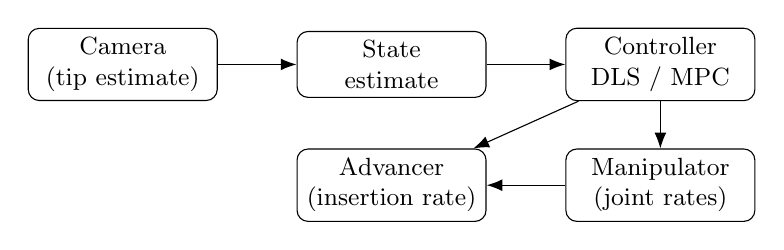
\begin{tikzpicture}[
  node distance=6mm and 10mm,
  box/.style={draw, rounded corners, align=center, minimum height=8mm, minimum width=24mm, font=\small},
  >={Latex[length=2mm]}
]
\node[box] (cam) {Camera\\(tip estimate)};
\node[box, right=of cam] (state) {State\\estimate};
\node[box, right=of state] (ctrl) {Controller\\DLS / MPC};
\node[box, below=of ctrl] (robot) {Manipulator\\(joint rates)};
\node[box, left=of robot] (adv) {Advancer\\(insertion rate)};
\draw[->] (cam) -- (state);
\draw[->] (state) -- (ctrl);
\draw[->] (ctrl) -- (robot);
\draw[->] (ctrl) -- (adv);
\draw[->] (robot.west) -- (adv.east);
\end{tikzpicture}
\caption{Closed-loop architecture. Vision, manipulator joint state and
insertion length are fused into a single state estimate each control tick;
the active controller maps this and the offline reference trajectory to
joint and insertion rate commands.}
\label{fig:architecture}
\end{figure}

\subsection{Magnetic Beam Model}
\label{sec:beam-model}

\subsubsection{Kinematics and constitutive model}
The beam is modeled as a Cosserat rod of inserted length $\ell$ and
circular cross section, following geometrically exact rod
theory~\cite{rucker2010geometrically} under a piecewise-constant-strain
(PCS) discretization~\cite{renda2018discrete}: the centerline is divided
into $n_s$ nodes, and the local strain
$u(s)=[u_1(s);u_2(s);u_3(s)]$ --- one torsion and two bending curvatures,
expressed in the body frame --- is constant on each of the $n_s-1$
segments. The material is linear elastic with cross-sectional stiffness
\begin{equation}
K = \operatorname{diag}\big(G I_p,\ E I,\ E I\big),
\label{eq:stiffness}
\end{equation}
where $E$ and $G=E/(2(1+\nu))$ are the composite Young's and shear moduli
for Poisson's ratio $\nu$, and $I$, $I_p$ are the second and polar moments
of area. Given the strain field, the centerline pose $(p(s),R(s))$ follows
from the rod reconstruction equations
\begin{equation}
p'(s) = R(s)\,e_3, \qquad R'(s) = R(s)\,\widehat{u(s)},
\label{eq:reconstruction}
\end{equation}
integrated from the fixed insertion point, with $\widehat{(\cdot)}$ the
skew-symmetric operator.

\subsubsection{Magnetic actuation}
Under (A3) the actuating magnet is an ideal point dipole of moment $m_a$
at position $p_a$, producing at a field point $x$
\begin{equation}
B(x;\theta) = \frac{\mu_0}{4\pi\lVert \Delta\rVert^{3}}
\Big(3(\hat{\Delta}\cdot m_a)\,\hat{\Delta} - m_a\Big),
\quad \Delta = x-p_a,\ \hat{\Delta}=\frac{\Delta}{\lVert\Delta\rVert},
\label{eq:dipole-field}
\end{equation}
the standard dipole model used throughout the magnetic continuum robot
literature~\cite{fu2023magnetic,kratchman2017guiding}. Under (A2) the beam
carries a hard-magnetized moment density $m(s)$, fixed in the body frame,
so that its world-frame moment at arclength $s$ is $R(s)m(s)$ and the
magnetic potential energy is
\begin{equation}
W_m[u;\theta] = -\int_0^{\ell} \big(R(s)m(s)\big)\cdot
B\big(p(s);\theta\big)\,ds,
\label{eq:magnetic-energy}
\end{equation}
evaluated at segment midpoints under the PCS discretization.

\subsubsection{Quasi-static equilibrium}
The elastic energy of the deformed rod is
\begin{equation}
W_{el}[u] = \tfrac12\int_0^{\ell}\big(u(s)-u^{\circ}\big)^{\!\top} K
\big(u(s)-u^{\circ}\big)\,ds,
\label{eq:elastic-energy}
\end{equation}
with $u^{\circ}$ the rest strain (zero for an initially straight beam).
The model additionally supports a gravitational term
$W_g[u]=\int_0^{\ell}\rho A\,g\cdot p(s)\,ds$, for mass per unit length
$\rho A$ and gravity vector $g$, and a lumen-contact penalty $W_{cf}[u]$
for operation inside a confining tube of local radius $R_\text{lum}(s)$.
Writing $\delta(s)$ for the distance from the beam centerline to the lumen
centerline and $r_b$ for the beam radius, the penetration
$\varphi(s)=\delta(s)+r_b-R_\text{lum}(s)$ enters through a smoothed
one-sided quadratic penalty
\begin{equation}
\varphi_+(s)=\tfrac12\Big(\varphi(s)+\sqrt{\varphi(s)^2+\epsilon^2}\Big),
\quad
W_{cf}[u]=\int_0^{\ell}\tfrac12 k_c\,\varphi_+(s)^2\,ds,
\label{eq:contact-energy}
\end{equation}
with contact stiffness $k_c$ and smoothing parameter $\epsilon$. Both
terms are retained for generality; the free-space, horizontally supported
configuration considered in this work sets $W_g\equiv W_{cf}\equiv 0$. The
total potential energy is
\begin{equation}
\Pi(u;\theta) = W_{el}[u] + W_m[u;\theta] + W_g[u] + W_{cf}[u],
\label{eq:total-energy}
\end{equation}
and, by (A1), the beam shape at a given input is its minimizer
\begin{equation}
u^{*}(\theta) = \operatorname*{arg\,min}_{u}\ \Pi(u;\theta).
\label{eq:equilibrium}
\end{equation}
Equation~\eqref{eq:equilibrium} is solved by bound-constrained quasi-Newton
minimization (L-BFGS-B~\cite{byrd1995lbfgsb}) on analytic energy
gradients. Because insertion is physically incremental, the solve uses
quasi-static continuation in $\ell$: the equilibrium at one insertion
length warm-starts the next, which accelerates convergence and prevents
the non-convex energy from admitting equilibria unreachable by the
physical insertion sequence. The regulated output is the tip pose
\begin{equation}
y(\theta) = \big[\,p(\ell);\ R(\ell)e_3\,\big]\in\mathbb{R}^6,
\label{eq:output}
\end{equation}
i.e.\ tip position and tip tangent.

\subsection{Control Jacobian}
\label{sec:jacobian}

Both the planner (Sec.~\ref{sec:planner}) and the controllers
(Sec.~\ref{sec:control}) require the sensitivity of the output
\eqref{eq:output} to the input, $J_b(\theta)=\partial y/\partial\theta$.
Rather than re-solving \eqref{eq:equilibrium} repeatedly under finite
perturbations, $J_b$ is obtained by implicit differentiation of the
equilibrium condition. Differentiating $\nabla_u\Pi(u^{*};\theta)=0$ with
respect to $\theta$ gives
\begin{equation}
\Pi_{uu}\,\frac{\partial u^{*}}{\partial\theta} + \Pi_{u\theta} = 0
\ \Longrightarrow\
\frac{\partial u^{*}}{\partial\theta} = -\,\Pi_{uu}^{-1}\,\Pi_{u\theta},
\label{eq:ift}
\end{equation}
where $\Pi_{uu}$ and $\Pi_{u\theta}$ denote the second derivatives of the
total energy at equilibrium, evaluated by finite differencing of the
analytic energy gradient. The beam Jacobian follows by the chain rule,
\begin{equation}
J_b(\theta) = \frac{\partial y}{\partial u}
\frac{\partial u^{*}}{\partial\theta}
+ \left.\frac{\partial y}{\partial\theta}\right\rvert_{u=u^{*}}
\in\mathbb{R}^{6\times7},
\label{eq:jacobian-chain}
\end{equation}
the second term capturing the explicit dependence of the forward
kinematics on $\theta$ at fixed strain, e.g.\ through $\ell$. This
implicit route contrasts with the finite-difference Jacobian obtained from
repeated boundary-value solves in~\cite{kratchman2017guiding}, and with
the analytic sensitivity boundary-value problem of~\cite{wu2025closedloop},
which is formulated around a shooting rather than an energy-minimization
solution.

Because the magnet pose is realized by the manipulator, the full
configuration-space Jacobian is
\begin{equation}
J(z) = J_b\big(\theta(z)\big)\,
\operatorname{blkdiag}\!\big(J_r(q),\,1\big)\in\mathbb{R}^{6\times7},
\label{eq:full-jacobian}
\end{equation}
where $J_r(q)\in\mathbb{R}^{6\times6}$ is the manipulator Jacobian,
computed in closed form rather than by finite differencing: for joint $i$
with axis $a_i$ and origin $o_i$ in the base frame, obtained from the
Denavit--Hartenberg product of transforms, the geometric Jacobian columns
are the standard revolute expressions~\cite{lynchpark2017modern}
\begin{equation}
J_r(q)\big[:,i\big] =
\begin{bmatrix} a_i\times(p_e-o_i)\\ a_i\end{bmatrix},
\label{eq:robot-jacobian}
\end{equation}
with $p_e$ the end-effector origin. The same per-robot calibrated
Denavit--Hartenberg parameters are used for \eqref{eq:robot-jacobian} and
for the forward kinematics, so that the calibrated positioning accuracy of
the arm carries over to the control Jacobian used by the planner and both
controllers.

$J(z)$ is severely ill-conditioned: only a low-dimensional subspace of the
seven-dimensional configuration space produces appreciable tip motion, a
direct consequence of the limited lateral steering authority available
from a single external magnet. Comparable rank deficiency is reported for
related single-magnet systems~\cite{kratchman2017guiding}. This property
motivates the explicit treatment of near-singular directions in both
controllers below.

\subsection{Offline Reference Trajectory Generation}
\label{sec:planner}

A reference trajectory is generated offline in two stages and supplied to
both controllers as a feedforward term.

\subsubsection{Geometric path}
Waypoint configurations $\chi_j=[q;\ell]_j$ are obtained sequentially by
nonlinear least squares on the residual
\begin{equation}
r(\chi_j) =
\begin{bmatrix}
\big(p_{\mathrm{tip}}(\chi_j)-p_{\mathrm{des},j}\big)/\tau_p\\[2pt]
\big(t_{\mathrm{tip}}(\chi_j)-t_{\mathrm{des},j}\big)/\tau_t\\[2pt]
\sqrt{w_c}\,\big(\chi_j-\chi_{j-1}\big)/d_c\\[2pt]
\sqrt{w_0}\,\big(\chi_j-\chi_0\big)/d_0
\end{bmatrix},
\label{eq:planner-residual}
\end{equation}
whose blocks are, in order, the tip position and tangent errors normalized
by tolerances $\tau_p,\tau_t$; a continuity term penalizing departure from
the previous waypoint (weight $w_c$, scale $d_c$); and a regularizer
holding the redundant configuration near a nominal posture $\chi_0$
(weight $w_0$, scale $d_0$). Equation~\eqref{eq:planner-residual} is
minimized by a bound-constrained trust-region-reflective least-squares
solver with Jacobian scaling, supplied with the analytic Jacobian
\eqref{eq:full-jacobian} and convergence tolerances of $10^{-9}$ on cost,
step and gradient. Because the problem is non-convex and
\eqref{eq:full-jacobian} is ill-conditioned, each waypoint is attempted
from an ordered set of initial guesses --- the previous waypoint's solution
extrapolated forward, followed by randomly perturbed restarts --- and the
first converged candidate is accepted. Acceptance is not delegated to the
optimizer's convergence flag: each candidate is re-validated by
re-evaluating the full nonlinear forward model from that waypoint's frozen
continuation baseline before it is committed to the path.

\subsubsection{Time parameterization}
The geometric path is then time-parameterized by reachability-based
time-optimal path
parameterization~\cite{bobrow1985timeoptimal,shinmckay1985minimumtime,phampham2018reachability}.
With $\sigma$ the path parameter, $\beta=\dot\sigma^{2}$ and
$\alpha=\ddot\sigma$, a backward pass computes the controllable set and a
forward pass the maximum feasible speed profile, subject to per-joint and
insertion velocity and acceleration bounds scaled by a fixed safety factor
below their physical limits. The resulting timing law is smoothed by a
$C^2$ natural cubic spline to remove knot-velocity discontinuities, and
its duration is dilated to an exact multiple of the control period
$\Delta t$ so that reference samples align with control ticks. The stage
yields, for each reference sample $k$, a reference configuration $z^\star_k$
and a reference rate $v^\star_k$.

\subsection{Vision-Based Tip Estimation}
\label{sec:vision}

The measured tip position $p_k$ is produced by a single overhead camera
and a planar reconstruction consistent with (A4), running on a dedicated
thread decoupled from both the frame-grab thread and the control loop; the
controller consumes the most recent reconstruction at each tick.

Two marker colors serve distinct roles. Red markers identify tracked
points on the beam --- its base, one or more intermediate points, and the
tip --- and are detected by HSV thresholding with a dual hue-range test
accommodating the wraparound of red hues, followed by morphological
opening, contour extraction within a calibrated region of interest, and
area-filtered centroid extraction from image moments,
$\big(M_{10}/M_{00},\,M_{01}/M_{00}\big)$. A fixed pair of green markers,
separated by a known distance $d_{\mathrm{cal}}$, is not tracked per frame
but provides the pixel-to-metric scale
$\gamma = d_{\mathrm{cal}}/\lVert g_1-g_2\rVert_{\mathrm{px}}$.

Reconstruction is planar rather than a full triangulation or
perspective-$n$-point solve. Three proximal red markers define a local
beam frame by principal component analysis: the axial axis is the leading
singular vector of the centered marker coordinates, sign-disambiguated
against the base-to-tangent direction, with the lateral axis completing
the orthonormal pair. Each detected marker, including the tip, is
projected onto this frame, scaled by $\gamma$, and embedded with zero
out-of-plane component as
$p_{\mathrm{local}}=[\,\xi,\ \zeta,\ 0\,]^{\top}$. A fixed, separately
calibrated rigid transform about the insertion point maps this into the
manipulator base frame,
$p_k = T_{\mathrm{piv}}\,p_{\mathrm{local}}$. The estimate is used
unfiltered.

\subsection{Closed-Loop Control}
\label{sec:control}

Both controllers track the reference $\{z^\star_k,v^\star_k\}$ and reuse
$v^\star_k$ as feedforward, correcting only the residual rather than
re-deriving the trajectory online. At control step $k$, $z_k$ is the
measured configuration, $p_k$ the measured tip position,
$p^\star_{k+1}$ the next reference tip position, and
$e_k = p^\star_{k+1}-p_k$ the tracking error.

\subsubsection{Damped least-squares controller}
\label{sec:dls}
The baseline controller re-evaluates the Jacobian at the measured
configuration at every tick, $J_k=J(z_k)$, and inverts it with Tikhonov
regularization~\cite{nakamura1986inverse,wampler1986manipulator}
\begin{equation}
J_k^{+} = J_k^{\top}\big(J_kJ_k^{\top}+\lambda^{2}I\big)^{-1},
\label{eq:dls}
\end{equation}
the damping $\lambda$ trading tracking accuracy against command magnitude
near singularities~\cite{chiaverini1994review}. Redundancy is resolved by
projecting a posture term and the feedforward rate into the null space of
$J_k$~\cite{liegeois1977automatic}, so that neither perturbs the tracked
output:
\begin{equation}
v_k = J_k^{+}\frac{k_p e_k}{\Delta t}
+ \big(I-J_k^{+}J_k\big)
\left(\frac{k_n\big(z^\star_k-z_k\big)}{\Delta t} + v^\star_k\right).
\label{eq:dls-full}
\end{equation}
The command is then limited in sequence by a velocity bound, an
acceleration bound relative to the previous command, and the
configuration box, with a final velocity re-clip. An anisotropic variant,
replacing the isotropic $\lambda^2 I$ in \eqref{eq:dls} with a
singular-value-dependent penalty from the decomposition of $J_k$, is
available but inactive in the present implementation.

\subsubsection{Output-tracking model predictive controller}
\label{sec:mpc}
The predictive controller models the configuration over an $N$-step
horizon as a single integrator, $z_{k+i+1}=z_{k+i}+\Delta t\,v_{k+i}$,
condensed onto the stacked command
$V=[v_k;\dots;v_{k+N-1}]$ as
\begin{equation}
Z = \Phi z_k + S V,
\label{eq:condensed}
\end{equation}
with $S$ block lower triangular in $\Delta t\,I$ and $\Phi$ the stacking
matrix; $D$ denotes the first-difference operator on $V$. Linearizing the
output map about the reference gives the predicted tip error
\begin{equation}
\Delta Y = \bar J S V + c,
\qquad
\bar J = \operatorname{blkdiag}\big(J_k,\dots,J_{k+N-1}\big),
\label{eq:output-prediction}
\end{equation}
where $c$ stacks the predicted tip error under zero correction. Offset-free
tracking is obtained by including in $c$ a constant output-disturbance
estimate $\hat d_k = p_k - y\big(\theta(z_k)\big)$, the discrepancy between
the measured tip and the model prediction at the measured configuration,
held fixed across the horizon.

Two Jacobian schedules are considered. The linear time-invariant (LTI)
variant freezes $\bar J$ at a single reference sample for the whole run;
the linear time-varying (LTV) variant evaluates a schedule once, offline,
at each reference sample. Both therefore condition the prediction on the
planned trajectory rather than on the measured configuration, in contrast
to the per-tick re-evaluation of Sec.~\ref{sec:dls}.

The command is the solution of the convex quadratic program
\begin{align}
\min_{V}\ & \big(Z-Z^\star\big)^{\!\top}\bar Q\big(Z-Z^\star\big)
+ V^{\top}\bar R V + (DV)^{\top}\bar R_d (DV) \notag\\
&\quad + \Delta Y^{\top}\bar Q_p \Delta Y + V^{\top}\Lambda_{dd}V
+ \big(z_N-z^\star_N\big)^{\!\top} P \big(z_N-z^\star_N\big)
\label{eq:mpc-cost}\\
\text{s.t.}\ & v_{\min}\le v_{k+i}\le v_{\max},\notag\\
& \big\lVert v_{k+i}-v_{k+i-1}\big\rVert\le a_{\max}\Delta t,\notag\\
& z_{\min}\le z_{k+i}\le z_{\max},\qquad i=0,\dots,N-1,\notag
\end{align}
solved by operator splitting~\cite{osqp2020}, of which only $v_k$ is
applied before the horizon recedes. Here $\bar Q_p$ weights tip-output
tracking and is the primary objective, while $\bar R$ and $\bar R_d$
penalize command magnitude and command increments. The configuration-space
weight $\bar Q$ is deliberately small: driving the configuration towards
the planned trajectory duplicates both the feedforward term and the
output-tracking objective, and the three compete for the same command
budget. It is retained at a small positive value because the terminal
weight $P$, the solution of the discrete algebraic Riccati equation for
the prediction model under combined weight
$\bar Q + J_N^{\top}\bar Q_p J_N$, requires $\bar Q$ to keep that weight
full rank given the rank deficiency of $J$ noted in
Sec.~\ref{sec:jacobian}. The terminal term supplies a cost-to-go
approximation beyond the horizon; no terminal set is imposed and no
nominal stability guarantee is claimed for the nonlinear plant.
$\Lambda_{dd}$ is an optional anisotropic penalty on near-null command
directions, formed per horizon step from the decomposition
$J_{k+i}=U\Sigma\Psi^{\top}$ with a floor on the penalty weight to
preserve conditioning of the quadratic program; it is the predictive
counterpart of the anisotropic variant in Sec.~\ref{sec:dls} and is
likewise inactive in the present implementation.

Both controllers are subject to the same velocity, acceleration and
configuration bounds. They differ in how the bounds are enforced: the
damped least-squares law applies them as a sequence of post-hoc limits on
an already-computed command, whereas the predictive controller enforces
them as hard constraints within \eqref{eq:mpc-cost}.

\subsection{Real-Time Implementation}
\label{sec:online}

Both controllers execute inside a single multi-threaded process on the
workstation of Table~\ref{tab:hardware}, whose real-time kernel provides
deterministic loop timing. Camera-based tip estimation, manipulator joint
angles and advancer insertion length are fused into one state estimate per
tick, and each controller is presented to the runtime through a common
solver interface, making them interchangeable without altering the
surrounding system. A supervisor halts motion on stale vision, an
unresponsive worker thread, a manipulator protective stop, a commanded
pose outside the calibrated workspace, or a non-finite command.

The manipulator is addressed over its real-time data exchange interface at
its native rate, with a dedicated thread re-issuing the current joint
velocity command between control ticks and a watchdog stopping motion if
commands cease. The advancer is driven over a serial link by a stepper
controller. The outer perception-and-control loop --- vision
reconstruction, state estimation, and the controller solve --- runs at
$\Delta t$. All computation is performed on CPU. Timing and platform
parameters are listed in Table~\ref{tab:hardware}, model and controller
parameters in Table~\ref{tab:params}.

\begin{table}[t]
\centering
\caption{Platform and real-time timing parameters.}
\label{tab:hardware}
\small
\begin{tabular}{@{}ll@{}}
\toprule
Quantity & Value \\
\midrule
CPU & Intel Core i7-11700K, 8C/16T, 3.60\,GHz \\
Memory & 32\,GB \\
Operating system & Ubuntu 22.04 LTS \\
Kernel & Linux 5.15, \texttt{PREEMPT\_RT} \\
Manipulator & Universal Robots UR10e \\
Robot interface rate & 500\,Hz \\
Command-stream rate & 125\,Hz \\
Watchdog rate & 10\,Hz \\
Control period $\Delta t$ & 0.1\,s (10\,Hz) \\
Frame-grab rate & up to 250\,Hz \\
Advancer link & 115200\,baud, 50\,Hz dispatch \\
Advancer resolution & 0.166\,mm/step \\
\bottomrule
\end{tabular}
\end{table}

\begin{table}[t]
\centering
\caption{Model and controller parameters.}
\label{tab:params}
\small
\begin{tabular}{@{}ll@{}}
\toprule
Quantity & Value \\
\midrule
Beam nodes $n_s$ & 10 \\
Beam diameter & 2.0\,mm \\
Actuating magnet & N52 NdFeB, $100\times100$\,mm cylinder \\
MPC horizon $N$ & 15 \\
Configuration weight $\bar Q$ & $1\times10^{-3}$ \\
Output weight $\bar Q_p$ & $1.0$ at $0.5$\,mm error scale \\
Terminal cost $P$ & enabled (Riccati) \\
Anisotropic damping $\Lambda_{dd}$ & inactive \\
DLS damping $\lambda$ & $1\times10^{-3}$ \\
Marker calibration distance $d_{\mathrm{cal}}$ & 38\,mm \\
\bottomrule
\end{tabular}
\end{table}

\begin{thebibliography}{99}

\bibitem{fu2023magnetic}
Fu \emph{et al.}, ``A Magnetically Controlled Guidewire Robot System with
Steering and Propulsion Capabilities for Vascular Interventional
Surgery,'' \emph{Advanced Intelligent Systems}, 2023.
% VERIFY: authors, volume/issue/pages, DOI.

\bibitem{kratchman2017guiding}
L.~B.~Kratchman \emph{et al.}, ``Guiding Elastic Rods With a
Robot-Manipulated Magnet for Medical Applications,'' \emph{IEEE
Transactions on Robotics}.
% VERIFY: authors, year, volume/issue/pages, DOI.

\bibitem{wu2025closedloop}
Wu and Zhang, ``Closed-Loop Magnetic Control of Medical Soft Continuum
Robots for Deflection,'' \emph{IEEE/ASME Transactions on Mechatronics}.
% VERIFY: authors, year, volume/issue/pages, DOI.

\bibitem{rucker2010geometrically}
D.~C.~Rucker, B.~A.~Jones, and R.~J.~Webster~III, ``A Geometrically Exact
Model for Externally Loaded Concentric-Tube Continuum Robots,'' \emph{IEEE
Transactions on Robotics}, vol.~26, no.~5, pp.~769--780, 2010.
% VERIFY: pages/DOI.

\bibitem{renda2018discrete}
F.~Renda, F.~Boyer, J.~Dias, and L.~Seneviratne, ``Discrete Cosserat
Approach for Multisection Soft Manipulator Dynamics,'' \emph{IEEE
Transactions on Robotics}, vol.~34, no.~6, pp.~1518--1533, 2018.
% VERIFY: pages/DOI.

\bibitem{byrd1995lbfgsb}
R.~H.~Byrd, P.~Lu, J.~Nocedal, and C.~Zhu, ``A Limited Memory Algorithm
for Bound Constrained Optimization,'' \emph{SIAM Journal on Scientific
Computing}, vol.~16, no.~5, pp.~1190--1208, 1995.
% VERIFY: pages/DOI.

\bibitem{lynchpark2017modern}
K.~M.~Lynch and F.~C.~Park, \emph{Modern Robotics: Mechanics, Planning,
and Control}. Cambridge University Press, 2017.

\bibitem{nakamura1986inverse}
Y.~Nakamura and H.~Hanafusa, ``Inverse Kinematic Solutions With
Singularity Robustness for Robot Manipulator Control,'' \emph{ASME Journal
of Dynamic Systems, Measurement, and Control}, vol.~108, no.~3,
pp.~163--171, 1986.
% VERIFY: pages/DOI.

\bibitem{wampler1986manipulator}
C.~W.~Wampler, ``Manipulator Inverse Kinematic Solutions Based on Vector
Formulations and Damped Least-Squares Methods,'' \emph{IEEE Transactions
on Systems, Man, and Cybernetics}, vol.~16, no.~1, pp.~93--101, 1986.
% VERIFY: pages/DOI.

\bibitem{chiaverini1994review}
S.~Chiaverini, B.~Siciliano, and O.~Egeland, ``Review of the Damped
Least-Squares Inverse Kinematics With Experiments on an Industrial Robot
Manipulator,'' \emph{IEEE Transactions on Control Systems Technology},
vol.~2, no.~2, pp.~123--134, 1994.
% VERIFY: pages/DOI.

\bibitem{liegeois1977automatic}
A.~Li\'{e}geois, ``Automatic Supervisory Control of the Configuration and
Behavior of Multibody Mechanisms,'' \emph{IEEE Transactions on Systems,
Man, and Cybernetics}, vol.~7, no.~12, pp.~868--871, 1977.
% VERIFY: pages/DOI.

\bibitem{bobrow1985timeoptimal}
J.~E.~Bobrow, S.~Dubowsky, and J.~S.~Gibson, ``Time-Optimal Control of
Robotic Manipulators Along Specified Paths,'' \emph{International Journal
of Robotics Research}, 1985.
% VERIFY: volume/issue/pages.

\bibitem{shinmckay1985minimumtime}
K.~G.~Shin and N.~D.~McKay, ``Minimum-Time Control of Robotic Manipulators
with Geometric Path Constraints,'' \emph{IEEE Transactions on Automatic
Control}, 1985.
% VERIFY: volume/issue/pages.

\bibitem{phampham2018reachability}
Q.-C.~Pham and D.~Pham, ``A New Approach to Time-Optimal Path
Parameterization Based on Reachability Analysis,'' \emph{IEEE
Transactions on Robotics}, vol.~34, no.~3, 2018.
% VERIFY: author initials/order, pages, DOI.

\bibitem{osqp2020}
B.~Stellato, G.~Banjac, P.~Goulart, A.~Bemporad, and S.~Boyd, ``OSQP: An
Operator Splitting Solver for Quadratic Programs,'' \emph{Mathematical
Programming Computation}, vol.~12, no.~4, pp.~637--672, 2020.
% VERIFY: pages/DOI.

\end{thebibliography}

\end{document}
